\documentclass[tikz,border=5pt]{standalone}
\usetikzlibrary{arrows.meta,positioning}
\begin{document}
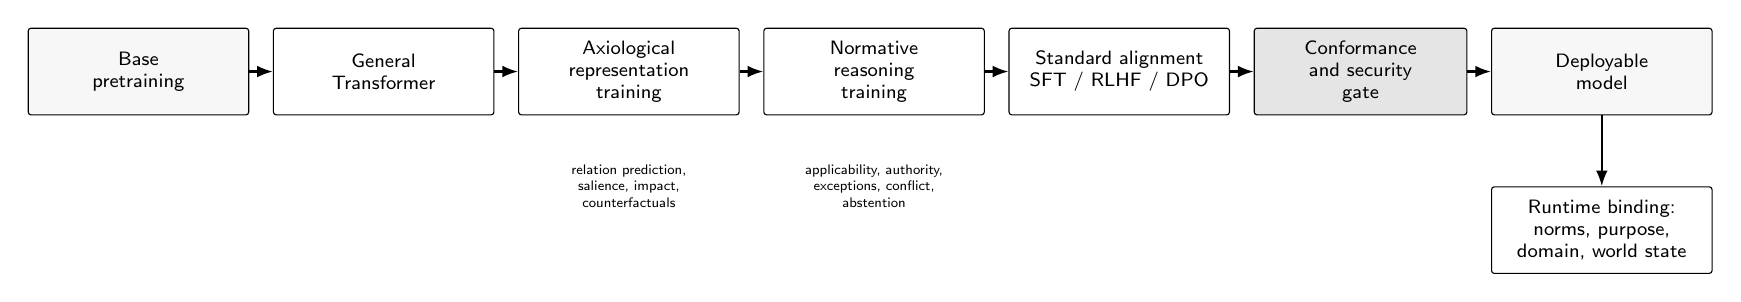
\begin{tikzpicture}[
  node distance=4mm and 3mm,
  box/.style={draw, rounded corners=1pt, minimum width=28mm, minimum height=11mm, align=center, font=\sffamily\scriptsize},
  gate/.style={draw, rounded corners=1pt, minimum width=27mm, minimum height=11mm, align=center, font=\sffamily\scriptsize, fill=black!10},
  arrow/.style={-{Latex[length=2mm]}, thick}
]
\node[box, fill=black!3] (pre) {Base\\pretraining};
\node[box, right=of pre] (base) {General\\Transformer};
\node[box, right=of base] (axi) {Axiological\\representation\\training};
\node[box, right=of axi] (norm) {Normative\\reasoning\\training};
\node[box, right=of norm] (align) {Standard alignment\\SFT / RLHF / DPO};
\node[gate, right=of align] (gate) {Conformance\\and security\\gate};
\node[box, right=of gate, fill=black!3] (deploy) {Deployable\\model};
\node[box, below=9mm of deploy] (runtime) {Runtime binding:\\norms, purpose,\\domain, world state};
\draw[arrow] (pre) -- (base);
\draw[arrow] (base) -- (axi);
\draw[arrow] (axi) -- (norm);
\draw[arrow] (norm) -- (align);
\draw[arrow] (align) -- (gate);
\draw[arrow] (gate) -- (deploy);
\draw[arrow] (deploy) -- (runtime);
\node[below=5mm of axi, align=center, font=\sffamily\tiny] {relation prediction,\\salience, impact,\\counterfactuals};
\node[below=5mm of norm, align=center, font=\sffamily\tiny] {applicability, authority,\\exceptions, conflict,\\abstention};
\end{tikzpicture}
\end{document}
